% Options for packages loaded elsewhere
\PassOptionsToPackage{unicode}{hyperref}
\PassOptionsToPackage{hyphens}{url}
%
\documentclass[
]{article}
\usepackage{amsmath,amssymb}
\usepackage{iftex}
\ifPDFTeX
  \usepackage[T1]{fontenc}
  \usepackage[utf8]{inputenc}
  \usepackage{textcomp} % provide euro and other symbols
\else % if luatex or xetex
  \usepackage{unicode-math} % this also loads fontspec
  \defaultfontfeatures{Scale=MatchLowercase}
  \defaultfontfeatures[\rmfamily]{Ligatures=TeX,Scale=1}
\fi
\usepackage{lmodern}
\ifPDFTeX\else
  % xetex/luatex font selection
\fi
% Use upquote if available, for straight quotes in verbatim environments
\IfFileExists{upquote.sty}{\usepackage{upquote}}{}
\IfFileExists{microtype.sty}{% use microtype if available
  \usepackage[]{microtype}
  \UseMicrotypeSet[protrusion]{basicmath} % disable protrusion for tt fonts
}{}
\makeatletter
\@ifundefined{KOMAClassName}{% if non-KOMA class
  \IfFileExists{parskip.sty}{%
    \usepackage{parskip}
  }{% else
    \setlength{\parindent}{0pt}
    \setlength{\parskip}{6pt plus 2pt minus 1pt}}
}{% if KOMA class
  \KOMAoptions{parskip=half}}
\makeatother
\usepackage{xcolor}
\usepackage[margin=1in]{geometry}
\usepackage{graphicx}
\makeatletter
\newsavebox\pandoc@box
\newcommand*\pandocbounded[1]{% scales image to fit in text height/width
  \sbox\pandoc@box{#1}%
  \Gscale@div\@tempa{\textheight}{\dimexpr\ht\pandoc@box+\dp\pandoc@box\relax}%
  \Gscale@div\@tempb{\linewidth}{\wd\pandoc@box}%
  \ifdim\@tempb\p@<\@tempa\p@\let\@tempa\@tempb\fi% select the smaller of both
  \ifdim\@tempa\p@<\p@\scalebox{\@tempa}{\usebox\pandoc@box}%
  \else\usebox{\pandoc@box}%
  \fi%
}
% Set default figure placement to htbp
\def\fps@figure{htbp}
\makeatother
\setlength{\emergencystretch}{3em} % prevent overfull lines
\providecommand{\tightlist}{%
  \setlength{\itemsep}{0pt}\setlength{\parskip}{0pt}}
\setcounter{secnumdepth}{-\maxdimen} % remove section numbering
\usepackage{booktabs}
\usepackage{longtable}
\usepackage{array}
\usepackage{multirow}
\usepackage{wrapfig}
\usepackage{float}
\usepackage{colortbl}
\usepackage{pdflscape}
\usepackage{tabu}
\usepackage{threeparttable}
\usepackage{threeparttablex}
\usepackage[normalem]{ulem}
\usepackage{makecell}
\usepackage{xcolor}
\usepackage{bookmark}
\IfFileExists{xurl.sty}{\usepackage{xurl}}{} % add URL line breaks if available
\urlstyle{same}
\hypersetup{
  pdftitle={Class Activity 1},
  pdfauthor={Chloe Barnes},
  hidelinks,
  pdfcreator={LaTeX via pandoc}}

\title{Class Activity 1}
\author{Chloe Barnes}
\date{2025-09-06}

\begin{document}
\maketitle

{
\setcounter{tocdepth}{2}
\tableofcontents
}
\section{Activity 1}\label{activity-1}

\subsection{1. Visualize the Data}\label{visualize-the-data}

\textbf{Visualize the pain ratings across the three drug formulations.
Provide a brief interpretation of what the graph reveals.}

\pandocbounded{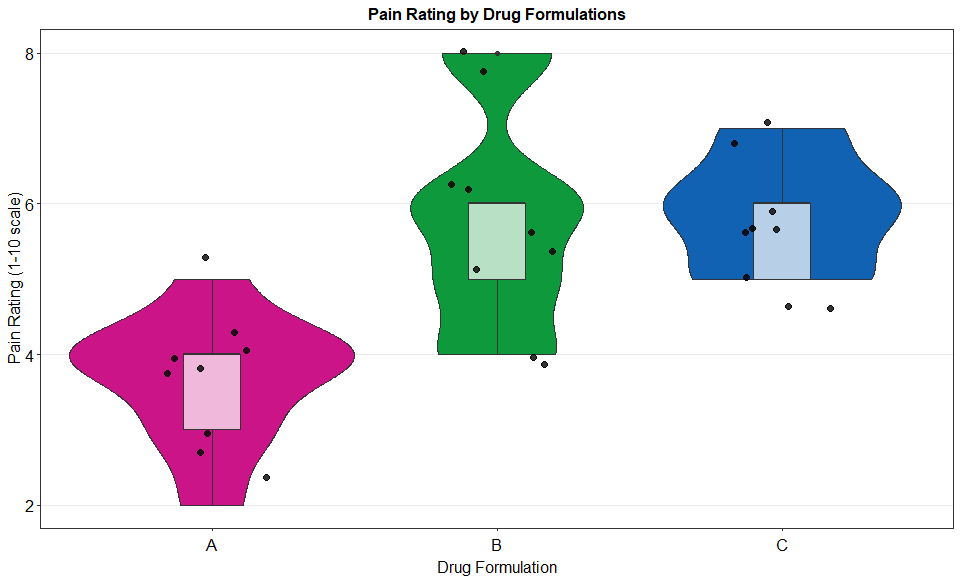
\includegraphics[keepaspectratio]{class_activity_1_part2_files/figure-latex/unnamed-chunk-3-1.pdf}}

From the graph, we see that Drug A appears to be the most effective, as
it has the lowest pain ratings. For Drug A, the median pain rating is
around 4, and the range of ratings are concentrated between 2 and 5. For
Drug B and Drug C, the medians are very similar at around 6. Drug B has
a wider spread than Drug C. The visualized data seems to suggest that
their may be differences in the the performance of Drug A vs.~Drug B.

\subsection{2. Statistical Analyses}\label{statistical-analyses}

\textbf{As the Data Scientist on a team of researchers at the
pharmaceutical company, your main task is to evaluate which drug
formulation most effectively reduces migraine pain. Formulate the
appropriate hypotheses, perform the relevant statistical test(s), and
communicate each step of your analysis and results in clear, accessible
written language for non-technical team members.}

\textbf{1. Study question:}

\begin{verbatim}
Do the three drug formulations differ in their effectiveness for reducign migraine pain?
\end{verbatim}

\textbf{2. Hypotheses}

\begin{itemize}
\item
  Null Hypothesis (H\textsubscript{0}):

  The average pain ratings are the same across all three drug
  formaulations. \({\mu}_A = {\mu}_B = {\mu}_C\)
\item
  Alternative Hypothesis (H\textsubscript{A}):

  At least one formulation has a different average pain rating. Not all
  group means are equal.
\end{itemize}

\textbf{3. Statistical Testing}

\begin{itemize}
\item
  I will use the One-Way ANOVA (Analysis of Variance) test because we
  are comparing three groups simultaneously.

  \textbf{Key Assumptions:}

  \begin{enumerate}
  \def\labelenumi{\arabic{enumi}.}
  \tightlist
  \item
    Independence: Each response is independent
  \item
    Normality: Pain ratings are approximately normally distributed
  \item
    Equal Variance: Variability is similar across groups
  \end{enumerate}
\end{itemize}

\begin{verbatim}
##             Df Sum Sq Mean Sq F value   Pr(>F)    
## Drug         2  28.22  14.111   11.91 0.000256 ***
## Residuals   24  28.44   1.185                     
## ---
## Signif. codes:  0 '***' 0.001 '**' 0.01 '*' 0.05 '.' 0.1 ' ' 1
\end{verbatim}

From the ANOVA test, F = 11.91 and p = 0.000256.

Because p \textless{} 0.05, there are statistically significant
differences between the three drug formulations.

\textbf{4. Post-hoc Tests}

Because the ANOVA test indicated a significant result, I will use a
Post-hoc Tukey HSD test to identify which specific groups are different
from each other.

\pandocbounded{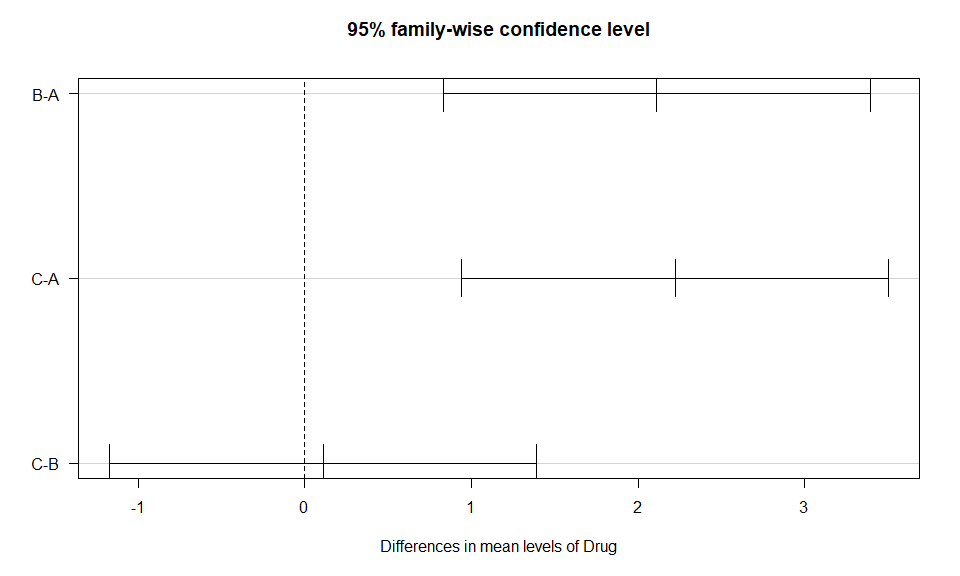
\includegraphics[keepaspectratio]{class_activity_1_part2_files/figure-latex/unnamed-chunk-5-1.pdf}}

\begin{verbatim}
##   Tukey multiple comparisons of means
##     95% family-wise confidence level
## 
## Fit: aov(formula = Pain_Rating ~ Drug, data = trial_data)
## 
## $Drug
##          diff        lwr      upr     p adj
## B-A 2.1111111  0.8295028 3.392719 0.0011107
## C-A 2.2222222  0.9406139 3.503831 0.0006453
## C-B 0.1111111 -1.1704972 1.392719 0.9745173
\end{verbatim}

The test shows that the difference of means for the B-A comparison and
the C-A comparison are both statistically significant because the
confidence intervals exclude 0 for both comparisons. The difference of
means of C-B is not statistically significant because 0 is included in
the confidence interval.

\textbf{5. Results and Interpretation}

\begin{itemize}
\tightlist
\item
  Patients taking Drug A consistently reported lower pain ratings
  compared to those on Drug B or C
\item
  There is no meaningful difference between Drug B or C
\item
  This means Drug A is the most effective at reducing migraine pain
\item
  \textbf{What this means:} The analysis shows that Drub A outperforms
  both Drug B and C in reducing migraine pain.
\item
  \textbf{How confident are we?} We are very confident. The results are
  statistically significant, meaning the differences are highly unlikely
  to be due to random chance
\item
  \textbf{Next Steps:} Based on these findings, further research and
  trials should prioritize Drug A as the leading candidate for
  development
\end{itemize}

\subsection{3. Discussion}\label{discussion}

\textbf{Suppose we wanted to build a supervised learning model using
this dataset. What would be the prediction goal? Discuss in what
situations a pharmaceutical company might prioritize inference over
prediction, and vice versa.}

\textbf{1. Prediction Goal} If we wanted to build a supervised learning
model, the goal would be to predict patient pain rating (1-10 scale)
given inputs such as:

\begin{itemize}
\tightlist
\item
  Which drug formulation was administered (A, B, or C)
\item
  Patient characteristics (is available) such as age, gender, migraine
  history, dosage, etc.
\item
  Prediction target (Y): Pain Rating
\item
  Coefficients (Features) (X): Drug Formulation and possibly other
  patient/clinical variables
\end{itemize}

\textbf{2. Inference vs.~Prediction}

\textbf{When to prioritize inference}

\begin{itemize}
\tightlist
\item
  a pharmaceutical company would prioritize inference when the goal is
  to understand \emph{why} and \emph{how} pain ratings differ between
  formulations
\item
  In this context, the pharmaceutical company may want to identify the
  most effective formulation, estimate the size of the effect (e.g
  ``Drug A lowers pain scores by \textasciitilde2 points compared to
  Drug B''), and/or provide scientific justification for regulatory
  approval (e.g.~the FDA)
\item
  In this case, inference would emphasize causality and statistical
  significance.
\end{itemize}

\textbf{When to prioritize prediction}

\begin{itemize}
\tightlist
\item
  a pharmaceutical company would prioritize prediction when the goal is
  to forecast an individual patient's pain outcome given their
  characteristics and the assigned drug.
\item
  In this context, the company may want to develop decision support
  tools for doctors (``Based on your patient's profile, which drug is
  likely to be most effective?'') and/or personalize treatments
\item
  In this case, prediction emphasizes accuracy for new cases, not just
  explanation.
\end{itemize}

\begin{verbatim}
## Dataset contains 548 observations and 7 variables
\end{verbatim}

\begin{verbatim}
## Campaigns: 3 2 1
\end{verbatim}

\begin{verbatim}
## Weeks: 1 2 3 4
\end{verbatim}

\begin{verbatim}
## Market Sizes: Small Medium Large
\end{verbatim}

\section{Activity 2}\label{activity-2}

\subsection{1. Exploratory Data
Analysis}\label{exploratory-data-analysis}

\subsubsection{Dataset Overview}\label{dataset-overview}

\begin{verbatim}
##     MarketID       MarketSize    LocationID      AgeOfStore    
##  Min.   : 1.000   Small : 60   Min.   :  1.0   Min.   : 1.000  
##  1st Qu.: 3.000   Medium:320   1st Qu.:216.0   1st Qu.: 4.000  
##  Median : 6.000   Large :168   Median :504.0   Median : 7.000  
##  Mean   : 5.715                Mean   :479.7   Mean   : 8.504  
##  3rd Qu.: 8.000                3rd Qu.:708.0   3rd Qu.:12.000  
##  Max.   :10.000                Max.   :920.0   Max.   :28.000  
##   Promotion             week           SalesInThousands
##  Length:548         Length:548         Min.   :17.34   
##  Class :character   Class :character   1st Qu.:42.55   
##  Mode  :character   Mode  :character   Median :50.20   
##                                        Mean   :53.47   
##                                        3rd Qu.:60.48   
##                                        Max.   :99.65
\end{verbatim}

\begin{verbatim}
## 'data.frame':    548 obs. of  7 variables:
##  $ MarketID        : int  1 1 1 1 1 1 1 1 1 1 ...
##  $ MarketSize      : Factor w/ 3 levels "Small","Medium",..: 2 2 2 2 2 2 2 2 2 2 ...
##  $ LocationID      : int  1 1 1 1 2 2 2 2 3 3 ...
##  $ AgeOfStore      : int  4 4 4 4 5 5 5 5 12 12 ...
##  $ Promotion       : chr  "3" "3" "3" "3" ...
##  $ week            : chr  "1" "2" "3" "4" ...
##  $ SalesInThousands: num  33.7 35.7 29 39.2 27.8 ...
\end{verbatim}

\subsubsection{Sales by Promotion}\label{sales-by-promotion}

\begin{longtable}[t]{lrrrr}
\caption{\label{tab:sales_by_promotion}Sales Summary by Campaign}\\
\toprule
Promotion & Mean\_Sales & Median\_Sales & SD\_Sales & Count\\
\midrule
Campaign 1 & 58.10 & 55.39 & 16.55 & 172\\
Campaign 2 & 47.33 & 45.39 & 15.11 & 188\\
Campaign 3 & 55.36 & 51.16 & 16.77 & 188\\
\bottomrule
\end{longtable}

\pandocbounded{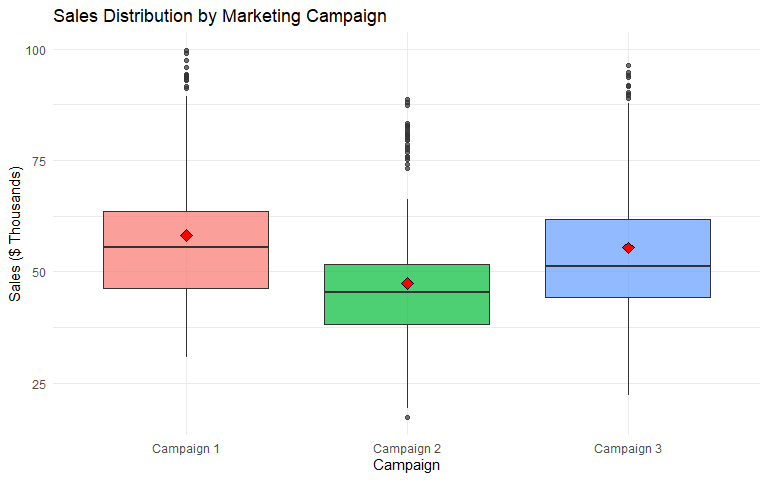
\includegraphics[keepaspectratio]{class_activity_1_part2_files/figure-latex/sales_by_promotion-1.pdf}}
\pandocbounded{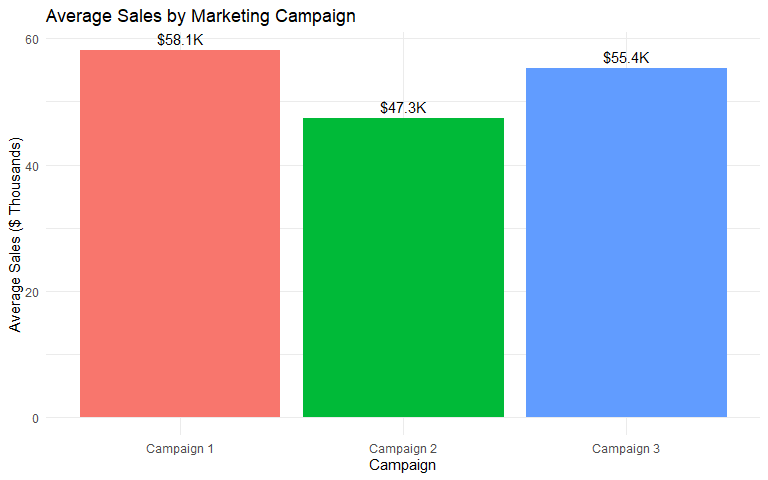
\includegraphics[keepaspectratio]{class_activity_1_part2_files/figure-latex/sales_by_promotion-2.pdf}}

Just observing the bar plot of average sales by marketing campaign, we
can make note that there may be possible differences in Sale by
Promotion. Campaign 2 appears to have a lower average sales (\$47.3K)
than compared to the other two campaigns (\$58.1K for Campaign 1 and
\$55.4K for Campaign 2). This will require more testing to confirm.

\subsubsection{Weekly Sales Trends Across
Promotions}\label{weekly-sales-trends-across-promotions}

\pandocbounded{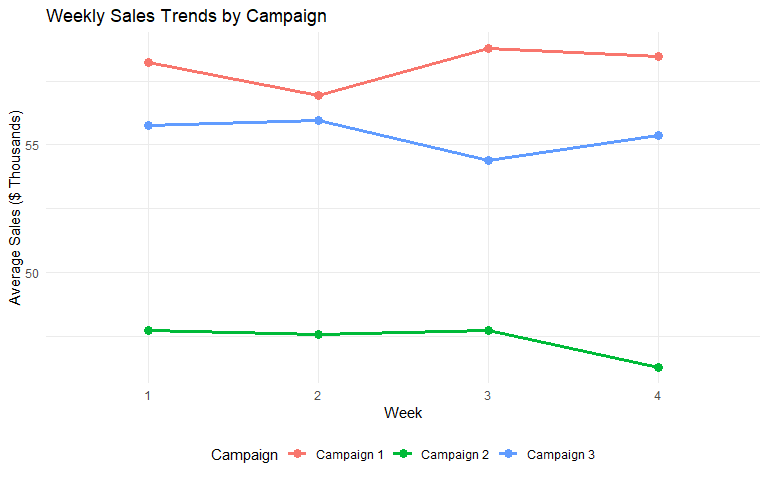
\includegraphics[keepaspectratio]{class_activity_1_part2_files/figure-latex/weekly_trends-1.pdf}}

\begin{longtable}[t]{lrrr}
\caption{\label{tab:weekly_trends}Average Sales by Week and Campaign}\\
\toprule
week & Campaign\_1 & Campaign\_2 & Campaign\_3\\
\midrule
1 & 58.24 & 47.73 & 55.78\\
2 & 56.93 & 47.58 & 55.95\\
3 & 58.77 & 47.72 & 54.38\\
4 & 58.45 & 46.28 & 55.35\\
\bottomrule
\end{longtable}

From the line plot, we again can observe potential differences in
average sales by campaign when accounting for weekly sales trends.
Campaign 2 appears to have much lower sales than campaign 1 or 3.
Campaign 1 appears to consistently have higher sales across all four
weeks of Promotion. This prompts further testing.

\subsubsection{Sales by Market Size}\label{sales-by-market-size}

\begin{longtable}[t]{lrrrr}
\caption{\label{tab:sales_by_market_size}Sales Summary by Market Size}\\
\toprule
MarketSize & Mean\_Sales & Median\_Sales & SD\_Sales & Count\\
\midrule
Small & 57.41 & 57.56 & 6.63 & 60\\
Medium & 43.99 & 44.59 & 9.05 & 320\\
Large & 70.12 & 75.02 & 17.05 & 168\\
\bottomrule
\end{longtable}

\pandocbounded{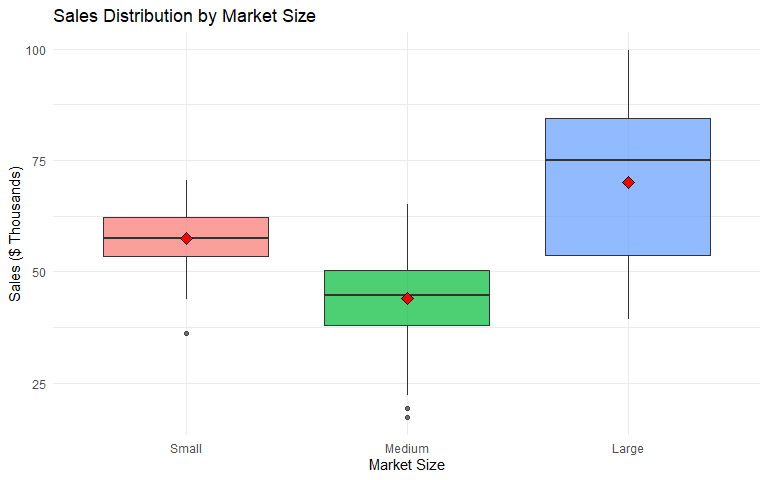
\includegraphics[keepaspectratio]{class_activity_1_part2_files/figure-latex/sales_by_market_size-1.pdf}}
\pandocbounded{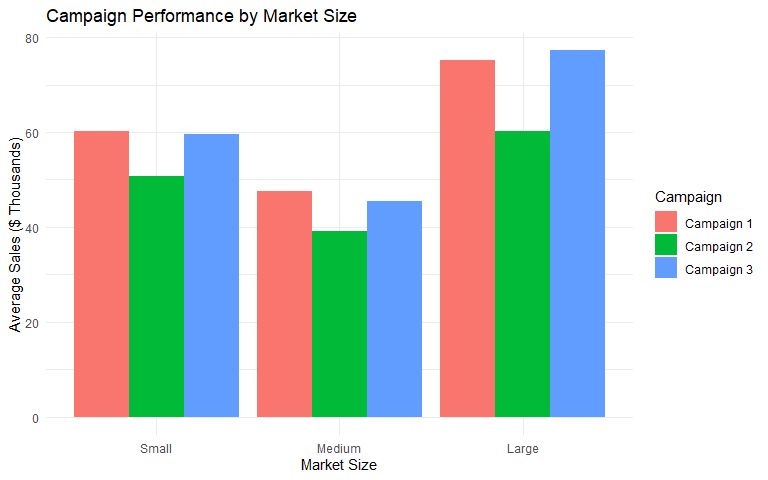
\includegraphics[keepaspectratio]{class_activity_1_part2_files/figure-latex/sales_by_market_size-2.pdf}}

\subsubsection{Additional Exploratory
Analysis}\label{additional-exploratory-analysis}

\pandocbounded{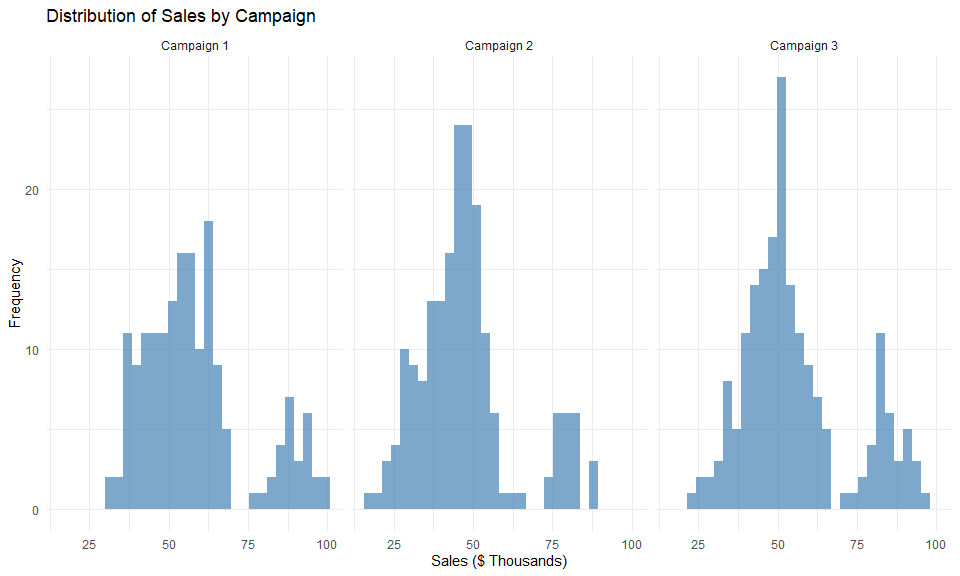
\includegraphics[keepaspectratio]{class_activity_1_part2_files/figure-latex/additional_eda-1.pdf}}

By looking at the distributions of sales by Campaign, it calls into
question the normality assumption of our data. The distributions appear
bi-modal. We should test for normality before running further
statistical tests, as this can affect our approach to the data.

\subsection{2. Research Questions and Statistical
Inference}\label{research-questions-and-statistical-inference}

\subsubsection{Research Question 1: Campaign
Effectiveness}\label{research-question-1-campaign-effectiveness}

\textbf{Question}: Do the three marketing campaigns differ significantly
in their sales performance?

\textbf{Hypotheses}:

\begin{itemize}
\tightlist
\item
  H₀: μ₁ = μ₂ = μ₃ (no significant difference between campaign means)
\item
  H₁: At least one campaign mean differs significantly from the others
\end{itemize}

\textbf{Normality Test}:

\begin{verbatim}
## 
##  Shapiro-Wilk normality test
## 
## data:  residuals(campaign_anova)
## W = 0.92208, p-value = 3.155e-16
\end{verbatim}

From the Shapiro-Wilk normality test, we got a p-value of 3.155e-16,
which is less than 0.05. This tells us that the normality assumption
would be incorrect an we should not assume the data is normally
distributed. We should use non-parametric methods to test the data.

\textbf{Statistical Testing}

\begin{verbatim}
## 
##  Kruskal-Wallis rank sum test
## 
## data:  SalesInThousands by Promotion
## Kruskal-Wallis chi-squared = 53.295, df = 2, p-value = 2.674e-12
\end{verbatim}

\begin{verbatim}
##   Comparison         Z      P.unadj        P.adj
## 1      1 - 2  7.024136 2.153947e-12 6.461842e-12
## 2      1 - 3  1.971891 4.862200e-02 4.862200e-02
## 3      2 - 3 -5.168403 2.361023e-07 4.722046e-07
\end{verbatim}

\textbf{Findings}:

The Kruskal-Wallis test indicated differences among campaigns (p =
2.674e-12, which is less than 0.05). I next performed Dunn pairwise
tests to compare Campaigns and determine which ones were different. The
output showed:

\begin{itemize}
\tightlist
\item
  Campaign 1 vs 2: Z = 7.02, p\_adj = 6.46×10⁻¹² → Campaign 1
  \textgreater{} Campaign 2.
\item
  Campaign 2 vs 3: Z = −5.17, p\_adj = 4.72×10⁻⁷ → Campaign 3
  \textgreater{} Campaign 2.
\item
  Campaign 1 vs 3: Z = 1.97, p\_adj = 0.0486 → Campaign 1 ≳ Campaign 3
  (small, borderline at α = 0.05).
\end{itemize}

\textbf{Interpretation}:

Campaign 2 under-performs both Campaigns 1 and 3 by a large margin.
Campaigns 1 and 3 are similar, with a modest edge for 1 that meets the
0.05 threshold.

\subsubsection{Research Question 2: Market Size and Campaign
Interaction}\label{research-question-2-market-size-and-campaign-interaction}

\textbf{Question}: Does campaign effectiveness vary by market size?

\textbf{Hypotheses}:

\begin{itemize}
\tightlist
\item
  H₀: No interaction between campaign type and market size
\item
  H₁: Campaign effectiveness varies significantly by market size
\end{itemize}

\textbf{Statistical Testing}

For this analysis, I used a Two-way ANOVA test

\begin{verbatim}
##                       Df Sum Sq Mean Sq F value  Pr(>F)    
## Promotion              2  11449    5725  49.611 < 2e-16 ***
## MarketSize             2  77803   38902 337.136 < 2e-16 ***
## Promotion:MarketSize   4   2117     529   4.586 0.00119 ** 
## Residuals            539  62194     115                    
## ---
## Signif. codes:  0 '***' 0.001 '**' 0.01 '*' 0.05 '.' 0.1 ' ' 1
\end{verbatim}

\begin{verbatim}
## # Effect Size for ANOVA (Type I)
## 
## Parameter            | Eta2 (partial) |       95% CI
## ----------------------------------------------------
## Promotion            |           0.16 | [0.11, 1.00]
## MarketSize           |           0.56 | [0.51, 1.00]
## Promotion:MarketSize |           0.03 | [0.01, 1.00]
## 
## - One-sided CIs: upper bound fixed at [1.00].
\end{verbatim}

\begin{verbatim}
## MarketSize = Small:
##  contrast                estimate   SE  df t.ratio p.value
##  Promotion1 - Promotion2    9.352 3.60 539   2.596  0.0262
##  Promotion1 - Promotion3    0.648 3.25 539   0.199  0.9783
##  Promotion2 - Promotion3   -8.704 3.47 539  -2.510  0.0330
## 
## MarketSize = Medium:
##  contrast                estimate   SE  df t.ratio p.value
##  Promotion1 - Promotion2    8.558 1.51 539   5.680  <.0001
##  Promotion1 - Promotion3    2.204 1.48 539   1.487  0.2980
##  Promotion2 - Promotion3   -6.355 1.44 539  -4.424  <.0001
## 
## MarketSize = Large:
##  contrast                estimate   SE  df t.ratio p.value
##  Promotion1 - Promotion2   14.914 1.97 539   7.588  <.0001
##  Promotion1 - Promotion3   -1.968 2.11 539  -0.931  0.6206
##  Promotion2 - Promotion3  -16.882 2.05 539  -8.231  <.0001
## 
## P value adjustment: tukey method for comparing a family of 3 estimates
\end{verbatim}

\pandocbounded{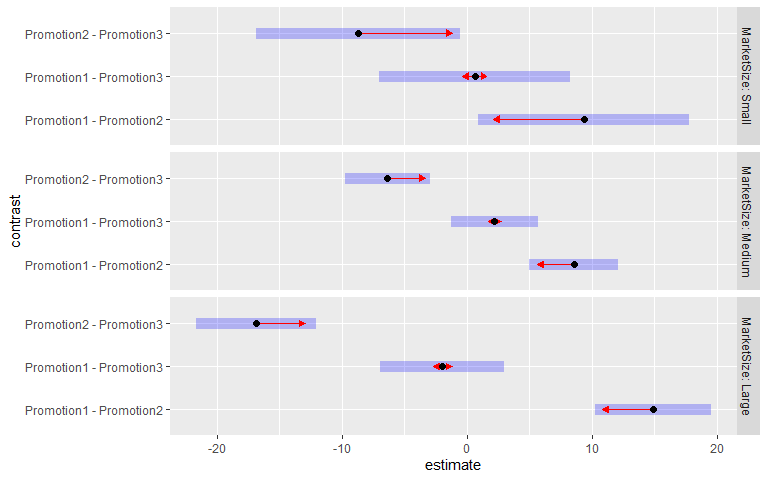
\includegraphics[keepaspectratio]{class_activity_1_part2_files/figure-latex/interaction_analysis-1.pdf}}
\pandocbounded{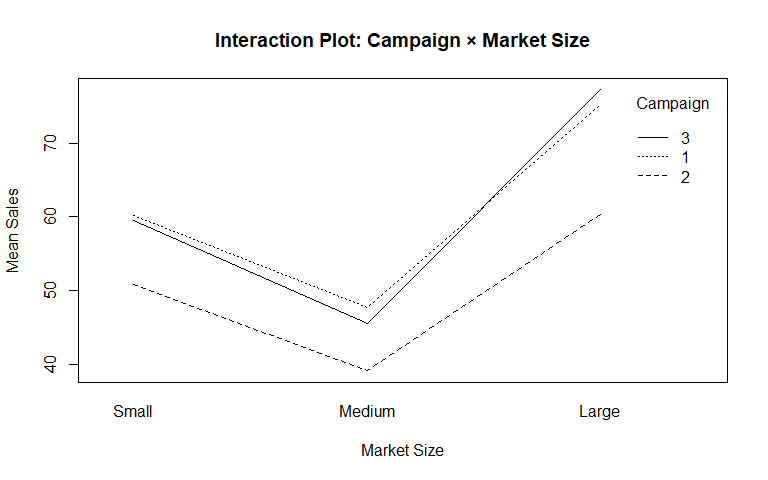
\includegraphics[keepaspectratio]{class_activity_1_part2_files/figure-latex/interaction_analysis-2.pdf}}

\textbf{Findings}: There were strong main effects of Promotion(F =
49.611, p \textless{} 2e-16) and MarketSize (F = 337.136 and p
\textless{} 2e-16), and a Promotion X MarketSize Interaction (F = 4.586,
p = 0.00119). This indicates the size of the campaign differences
changes across market sizes. Therefore, I examined simple effects
(Tukey-adjusted)

\begin{verbatim}
**Small Markets**

- 1 vs 2: +9.32, p = 0.026 --\> Campaign 1 \> Campaign 2
- 2 vs 3: -8.70, p = 0.033 --> Campaign 3 > Campaign 2
- 1 vs 3: +0.65, p = 0.978 --> Campaign 1 $\approx$ Campaign 3 (no difference)

**Medium Markets**
- 1 vs 2: +8.56, p < 0.0001 → Campaign 1 > 2
- 2 vs 3: −6.36, p < 0.0001 → Campaign 3 > 2
- 1 vs 3: +2.20, p = 0.298 → Camapign 1 ≈ Campaign 3 (no difference)

**Large Markets**
- 1 vs 2: +14.91, p < 0.0001 → Campaign 1 > 2
- 2 vs 3: −16.88, p < 0.0001 → Campaign 3 > 2
- 1 vs 3: -1.97, p = 0.621 → Camapign 1 ≈ Campaign 3 (point estimate favors 3 slightly, not significant)
\end{verbatim}

\textbf{Interpretation}:

Market size is the biggest driver of sales, but campaign choices still
matter. The interaction shows that how far ahead the better campaigns
are depends on market size. Across all market sizes, Campaign 2
under-performs both Campaigns 1 and 3 by substantial, statistically
significant margins. Campaigns 1 and 3 are statistically
indistinguishable within each market size.

\subsubsection{Research Question 3: Temporal
Stability}\label{research-question-3-temporal-stability}

\textbf{Question}: Does campaign effectiveness remain stable over the
4-week period?

\textbf{Hypotheses}:

\begin{itemize}
\tightlist
\item
  H₀: No significant change in campaign effectiveness over time
\item
  H₁: Campaign effectiveness changes significantly over time
\end{itemize}

\textbf{Statistical Testing}

\begin{verbatim}
##                 Df Sum Sq Mean Sq F value   Pr(>F)    
## Promotion        2  11449    5725  21.625 9.29e-10 ***
## week             3     24       8   0.030    0.993    
## Promotion:week   6    200      33   0.126    0.993    
## Residuals      536 141890     265                     
## ---
## Signif. codes:  0 '***' 0.001 '**' 0.01 '*' 0.05 '.' 0.1 ' ' 1
\end{verbatim}

\begin{verbatim}
## # A tibble: 12 x 3
##    week  Promotion Mean_Sales
##    <chr> <chr>          <dbl>
##  1 1     1               58.2
##  2 1     2               47.7
##  3 1     3               55.8
##  4 2     1               56.9
##  5 2     2               47.6
##  6 2     3               55.9
##  7 3     1               58.8
##  8 3     2               47.7
##  9 3     3               54.4
## 10 4     1               58.4
## 11 4     2               46.3
## 12 4     3               55.4
\end{verbatim}

\textbf{Findings}: The analysis shows no significant interaction between
Campaign and Week (p \textgreater{} 0.05), indicating that campaign
effectiveness remains stable over the 4-week test period.

\subsection{3. Statistical Inference vs.~Predictive
Modeling}\label{statistical-inference-vs.-predictive-modeling}

\subsubsection{Why Emphasize Statistical
Inference}\label{why-emphasize-statistical-inference}

For this fast-food chain's marketing campaign decision,
\textbf{statistical inference is more appropriate than predictive
modeling} for several key reasons:

\begin{itemize}
\tightlist
\item
  \textbf{Decision Goal}: The chain needs to select ONE campaign for
  chain-wide deployment
\item
  \textbf{Causal Understanding}: They need to understand WHY Campaign 1
  is better, not just predict future sales
\item
  \textbf{Risk Management}: Statistical significance provides confidence
  for large-scale investment decisions
\item
  \textbf{Stakeholder Communication}: P-values and confidence intervals
  are easily interpretable for executives
\end{itemize}

\paragraph{When Predictive Modeling Would Be
Useful}\label{when-predictive-modeling-would-be-useful}

Predictive modeling would be more appropriate for:

\begin{itemize}
\tightlist
\item
  Forecasting individual store sales
\item
  Optimizing campaign elements (timing, messaging, targeting)
\item
  Handling complex non-linear relationships
\item
  Real-time performance monitoring
\end{itemize}

\subsubsection{Market Size Influence on Promotion
Effectiveness}\label{market-size-influence-on-promotion-effectiveness}

\begin{longtable}[t]{llrrr}
\caption{\label{tab:market_size_analysis}Campaign Performance by Market Size}\\
\toprule
MarketSize & Promotion & Mean\_Sales & SD\_Sales & Count\\
\midrule
Small & 1 & 60.16 & 5.13 & 20\\
Small & 2 & 50.81 & 5.87 & 16\\
Small & 3 & 59.51 & 5.21 & 24\\
Medium & 1 & 47.67 & 8.07 & 96\\
Medium & 2 & 39.11 & 8.81 & 108\\
\addlinespace
Medium & 3 & 45.47 & 8.09 & 116\\
Large & 1 & 75.24 & 15.50 & 56\\
Large & 2 & 60.32 & 15.73 & 64\\
Large & 3 & 77.20 & 14.40 & 48\\
\bottomrule
\end{longtable}

\begin{verbatim}
## Large markets generate 58 % higher sales than medium markets
\end{verbatim}

\paragraph{How market size can shape effectiveness and
sales:}\label{how-market-size-can-shape-effectiveness-and-sales}

The ANOVA shows MarketSize is the dominant driver.

Mechanisms:

\begin{itemize}
\tightlist
\item
  Baseline demand/foot traffic: Larger markets have more potential
  buyers -\textgreater{} higher absolute sales and bigger headroom for
  lift
\item
  Media reach \& saturation: The same spend/creative scales better in
  larger markets
\item
  Competitive intensity: IN big markets, differentiated creatives may
  matter more. In small markets, relationships/local presence may be
  more important
\item
  Operational constraints: Stockouts or staffing can cap realized lift.
  Larger markets might be better staffed/supplied
\end{itemize}

\textbf{What I found}: Within Small and Medium markets, Campaigns 1 and
3 perform similarly and both beat campaign 2. In Large markets, the gap
between Campaigns 1/3 and 2 grows even more (there are bigger absolute
differences). The ranking is stable (2 under-performs everywhere), but
the size of the gap changes with MarketSize

\subsubsection{Store Age Influence on
Sales}\label{store-age-influence-on-sales}

\begin{longtable}[t]{llrr}
\caption{\label{tab:store_age_detailed}Campaign Performance by Store Age}\\
\toprule
AgeGroup & Promotion & Mean\_Sales & Count\\
\midrule
1-3 years & 1 & 67.67 & 48\\
1-3 years & 2 & 47.65 & 56\\
1-3 years & 3 & 66.70 & 28\\
4-6 years & 1 & 54.49 & 44\\
4-6 years & 2 & 42.53 & 28\\
\addlinespace
4-6 years & 3 & 53.08 & 52\\
7-9 years & 1 & 55.62 & 24\\
7-9 years & 2 & 50.06 & 44\\
7-9 years & 3 & 48.47 & 40\\
10+ years & 1 & 53.80 & 56\\
\addlinespace
10+ years & 2 & 47.27 & 60\\
10+ years & 3 & 56.49 & 68\\
\bottomrule
\end{longtable}

\begin{verbatim}
## Correlation between store age and sales: -0.029
\end{verbatim}

\paragraph{How Store age (AgeOfStore) could
matter}\label{how-store-age-ageofstore-could-matter}

Store age can be a proxy for multiple factors:

\begin{itemize}
\tightlist
\item
  Customer base maturity \& loyalty: Older stores often have established
  repeat customers, whereas newer stores may be more responsive to
  awareness-style campaigns.
\item
  Facility condition/location: Older store may be located in more
  well-known, high-traffic areas. Conversely, they may be located in
  aging retail corridors. Age can correlate with market demographics and
  with MarketSize (which can lead to potential confounding)
\end{itemize}

\textbf{What I found}:

Store age has a weak correlation with sales performance (r = -0.029).
For this analysis, chain-wide rollout of chosen campaign may be
appropriate regardless of store maturity.

\subsubsection{Conclusion and
Recommendations}\label{conclusion-and-recommendations}

Based on this statistical analysis:

Roll out Campaign 1 or 3 across sizes; avoid 2. The choice between 1 and
3 can be mode on creatie fit or cost since they are statistically
indistinguishable within each MarketSize.

\end{document}
